\documentclass[12pt, a4paper,oneside]{book}
\newcommand{\re}{\mathrm{e}}
\newcommand{\ri}{\mathrm{i}}
\newcommand{\rd}{\mathrm{d}}
\def\semicolon{\nobreak\mskip2mu\mathpunct{}\nonscript\mkern-\thinmuskip{;}
\mskip6muplus1mu\relax} % This defines the semicolon command

        % allows index generation
\usepackage{graphicx}        % standard LaTeX graphics tool
                             % when including figure files
\usepackage{multicol}        % used for the two-column index




\usepackage{color,tikz}
%\usepackage[unicode,bookmarks,bookmarksopen,bookmarksopenlevel=2,colorlinks,linkcolor=blue,citecolor=green]{hyperref}

\usepackage{amsmath,eucal,amssymb}
\usepackage{mathrsfs,graphicx,texdraw}
\usepackage{fancyhdr,framed}
\usepackage{tikz, tikz-3dplot}
\usepackage{tkz-euclide}
\usetikzlibrary{decorations.fractals}
\usetikzlibrary{decorations.footprints}




\usepackage{palatino}

\usepackage[latin1]{inputenc}

\usepackage[T1]{fontenc}
%\usepackage[dvips]{graphicx}
%\usepackage{times}


\definecolor{mygreen}{HTML}{622567} %%% Purple
\definecolor{Gray}{HTML}{333333} %%% Gray

\definecolor{myred}{HTML}{D55C19} %%%EssexOrange
\definecolor{myblue}{HTML}{007A87} %%%Seagrass
\definecolor{Mint}{HTML}{35C4B5} %%% Mint


\def\grole{\mathrel{\mathchoice {\vcenter{\offinterlineskip\halign{\hfil
$\displaystyle##$\hfil\cr>\cr\noalign{\vskip-1.5pt}<\cr}}}
{\vcenter{\offinterlineskip\halign{\hfil$\textstyle##$\hfil\cr
>\cr\noalign{\vskip-1.5pt}<\cr}}}
{\vcenter{\offinterlineskip\halign{\hfil$\scriptstyle##$\hfil\cr
>\cr\noalign{\vskip-1pt}<\cr}}}
{\vcenter{\offinterlineskip\halign{\hfil$\scriptscriptstyle##$\hfil\cr
>\cr\noalign{\vskip-0.5pt}<\cr}}}}}

\newenvironment{rcases}
  {\left.\begin{aligned}}
  {\end{aligned}\right\rbrace}

\newenvironment{lcases}
  {\left\lbrace\begin{aligned}}
  {\end{aligned}\right.}

\newtheorem{theorem}{Theorem}[section]
\newtheorem{lemma}[theorem]{Lemma}
\newtheorem{proposition}[theorem]{Proposition}
\newtheorem{corollary}[theorem]{Corollary}
\newtheorem{definition}[theorem]{Definition}
\newtheorem{example}[theorem]{Example}
\newtheorem{remark}[theorem]{Remark}

\newenvironment{proof}[1][Proof]{\begin{trivlist}
\item[\hskip \labelsep {\bfseries #1}]}{\end{trivlist}}
\newenvironment{solution}[1][Solution]{\begin{trivlist}
\item[\hskip \labelsep {\bfseries #1}]}{\end{trivlist}}

\newcommand{\qed}{\nobreak \ifvmode \relax \else
      \ifdim\lastskip<1.5em \hskip-\lastskip
      \hskip1.5em plus0em minus0.5em \fi \nobreak
      \vrule height0.75em width0.5em depth0.25em\fi}

\numberwithin{equation}{section}
\def\Ad{{\mbox{Ad}}}
\def\im{{\mbox{Im}}}
\def\Re{{\mbox{Re}\;}}
\def\ad{\mathrm{ad\,}}
\def\openone{\leavevmode\hbox{\small1\kern-3.3pt\normalsize1}}
\def\Res{\mathop{\mbox{Res}\,}\limits}
\def\biglb{\big[\hspace*{-.7mm}\big[}
\def\bigrb{\big]\hspace*{-.7mm}\big]}


\def\bigrbt{\mathop{\bigrb }\limits_{\widetilde{\;}}}
\def\biggrbt{\mathop{\biggrb }\limits_{\widetilde{\;}}}
\def\Bigrbt{\mathop{\Bigrb }\limits_{\widetilde{\;}}}
\def\Biggrbt{\mathop{\Biggrb }\limits_{\widetilde{\;}}}

\def\bPhi{\mathbf{\Phi}}
\def\bM{\mathbf{M}}
\def\bm{\mathbf{m}}
\def\bbbc{{\Bbb C}}
\def\bbbr{{\Bbb R}}
\def\bbbz{{\Bbb Z}}
\def\bbbs{{\Bbb S}}
\def\diag{\mbox{diag}\,}
\def\tr{\mbox{tr}\,}

\textwidth=17cm   \textheight=24.5cm \voffset=-2cm

\evensidemargin=-0.5cm \oddsidemargin=-0.5cm

 \renewcommand{\baselinestretch}{1.5}

%%%%%%%%fancy header%%%%%%%%%%%%%%%%%

\usepackage{fancyhdr}
\pagestyle{fancy}
\usepackage{calc}
\newlength{\pageoffset}
\setlength{\pageoffset}{0cm}% use whatever you like
\fancyheadoffset[LE,RO]{\pageoffset}
\renewcommand{\chaptermark}[1]{\markboth{#1}{}}
\renewcommand{\sectionmark}[1]{\markright{\thesection\ #1}}
\fancyhf{}
\fancyhead[LE]{\makebox[\pageoffset][l]{\thepage}\hfill\leftmark}
\fancyhead[RO]{\rightmark\hfill\makebox[\pageoffset][r]{\thepage}}
\fancypagestyle{plain}{%
    \fancyhead{} % get rid of headers
    \renewcommand{\headrulewidth}{0pt} % and the line
}

%%%%%%%%%%%%%%%%%%%%%%%%%%%%%%%%%%%%

\arraycolsep=2pt

%%%%Fancy Chapter%%%

%\usepackage{lmodern}
\usepackage{graphicx}
\usepackage{xcolor}
\usepackage{titlesec}
\usepackage{microtype}
\usepackage{lipsum}

%\definecolor{myblue}{RGB}{0,82,155}

\titleformat{\chapter}[display]
  {\normalfont\bfseries\color{myred}}
  {\filleft\hspace*{-60pt}%
    \rotatebox[origin=c]{90}{%
      \normalfont\color{black}\Large%
        \textls[180]{\textsc{\chaptertitlename}}%
    }\hspace{10pt}%
    {\setlength\fboxsep{0pt}%
    \colorbox{myred}{\parbox[c][3cm][c]{2.5cm}{%
      \centering\color{white}\fontsize{80}{90}\selectfont\thechapter}%
    }}%
  }
  {10pt}
  {\titlerule[2.5pt]\vskip3pt\titlerule\vskip4pt\LARGE\sffamily}

% hyperref should be loaded after all other packages
% aliascnt is needed to get \autoref (from hyperref) to work correctly with custom amsthm theorems
\usepackage{aliascnt}
\usepackage[colorlinks,linkcolor=myblue,citecolor=mygreen]{hyperref}



\begin{document}


\thispagestyle{empty}

\begin{minipage}{0.2\textwidth}
\centerline{
\includegraphics[width=.4\textwidth]{essex} }
\end{minipage}
\begin{minipage}{0.8\textwidth}

$ \qquad \qquad \qquad ${\LARGE \bf \sl University of Essex}

{\LARGE \bf School of Computer Science and Electronic Engineering}

\end{minipage}

\begin{center}

\noindent\textcolor{myred}{\rule{\linewidth}{4.8pt}}

\vspace{1cm}

{\LARGE \sc  CE901-7: MSc Project and Dissertation}

\vspace{1.5cm}

{\Huge{\color{myblue}  Automated Sleep Phase Detection: Unveiling the Night's Secrets with Machine Learning}}

\vspace{1.5cm}

{\Large \bf Priyanshu Banerjee}




\vspace{2.0cm}


\vspace{1.5cm}

{\Large {Supervisor:Dr. Vito de Feo} }

\vspace{.25cm}

\noindent\textcolor{myred}{\rule{\linewidth}{4.8pt}}

\vspace{1cm}
{\Large \today }\\[4pt]\
{\Large Colchester}
\end{center}
\newpage
\tableofcontents

\listoffigures
\listoftables
\chapter*{Abstract} % Creates an unnumbered chapter for the abstract
\addcontentsline{toc}{chapter}{Abstract} % Adds the abstract to the table of contents
\begin{abstract}
    This dissertation explores the application of machine learning algorithms in the classification of sleep stages using polysomnography (PSG) data. The study leverages advanced machine learning models, including XGBoost, CatBoost, SVM, and Logistic Regression, to analyze sleep data under two experimental conditions: one utilizing a reduced feature set derived from 4-channel data post-PCA, and the other employing a comprehensive 13-channel feature extraction. The methodology encompasses rigorous data preparation, cross-validation, and performance evaluation. The findings reveal that ensemble methods and SVM consistently outperform Logistic Regression, highlighting their potential as robust tools for sleep stage classification. This research not only contributes to the field of biomedical signal processing but also has implications for clinical practices in sleep medicine.
\end{abstract}
\chapter{Introduction}\label{ch:1}

Ever found yourself wondering about the mysterious voyage we embark on each night when we surrender to sleep? You're not alone. The world of slumber is a captivating realm, and within it, there's a dance of sleep phases REM, non-REM, and a whole lot more that's as intricate as it is essential to our well-being.
But here's the kicker: understanding these sleep phases isn't just a quirky fascination; it's a key to unlocking a treasure trove of insights into our physical and mental health. The thing is, figuring out the specifics of these sleep phases has been a bit like detective work in the dark. Traditional methods involving sleep tests and human interpretations are great but come with their own set of challenges. That's where our superhero, Machine Learning, swoops in.
So, imagine this dissertation as a flashlight in the dark, aimed at those elusive sleep phases. We're diving into the sweet spot where sleep science meets machine learning, with a mission: to build smart models that can read the language of sleep. Why? Because once we crack that code, we can open up new possibilities for understanding sleep patterns and, ultimately, improving our snooze game.
\section{Significance of Sleep Phase Differentiation:}\label{sec:1.1}
The sleep cycle, characterized by its nuanced stages, plays a pivotal role in various physiological functions. Non-REM sleep, encompassing lighter stages (N1 and N2) and deep slow-wave sleep (N3), is associated with essential processes such as physical restoration, immune system modulation, and hormone regulation. Conversely, REM sleep, distinguished by heightened brain activity and vivid dreaming, contributes significantly to cognitive functions, particularly memory consolidation.

Disturbances in the natural progression through these sleep phases have been linked to a spectrum of health issues, emphasizing the critical need for accurate identification and classification. Sleep disorders, ranging from insomnia to sleep apnea, often manifest as disruptions in the balance between REM and non-REM sleep. Thus, the ability to precisely delineate these phases holds promise for early diagnosis and targeted interventions.

\section{Limitations of Traditional Sleep Monitoring Techniques}\label{sec:1.2}

 Despite the wealth of information provided by PSG, its applicability beyond laboratory settings is constrained by logistical challenges. The necessity for specialized equipment and expert supervision, coupled with the subjectivity inherent in manual scoring, hinders scalability and accessibility in real-world scenarios. As such, there is a compelling call for innovative methodologies capable of accommodating the evolving landscape of sleep research.


\section{Integration of Machine Learning into Sleep Research:}\label{sec:1.3}

The emergence of machine learning as a transformative force across various disciplines has prompted its exploration in sleep research. Machine learning algorithms, capable of processing extensive datasets and identifying intricate patterns, offer a potential solution to the challenges posed by traditional monitoring methods. With the proliferation of wearable devices equipped with sensors capable of unobtrusive and continuous monitoring, the synergy between machine learning and sleep science is poised to revolutionize the field.

The application of machine learning to sleep phase detection involves the extraction of informative features from diverse physiological signals. By training models on labeled datasets and validating their performance against established benchmarks, the aim is to surpass human expertise in sleep stage scoring and overcome the limitations of traditional methods.

\section{Objectives of the Dissertation:}\label{sec:1.4}

Against this backdrop, the primary objectives of this dissertation become evident. Firstly, it seeks to comprehensively review existing literature on sleep phase detection, encompassing both traditional methodologies and recent advances involving machine learning. Secondly, it aims to contribute to the field by developing and evaluating machine learning models for automated sleep phase detection. The dissertation will navigate through the complexities of feature extraction, model training, and validation, with a critical eye on the practical implications of these methodologies in real-world applications.

By engaging in this academic exploration, we aspire to not only deepen our understanding of sleep dynamics but also to pave the way for scalable and accessible sleep monitoring solutions. The subsequent chapters will delve into the intricacies of the methodologies employed, the challenges encountered, and the implications of our findings in the broader context of sleep research.

In the pursuit of unraveling the mysteries of sleep through the lens of machine learning, we embark on a scientific journey that bridges the realms of data-driven methodologies and the nuanced intricacies of human sleep.

\section{Acknowledgments}\label{sec:1.5}
The successful completion of this dissertation is the result of collaborative efforts and dedication from multiple individuals who have contributed their expertise and time to this extensive project. We would like to express our sincere gratitude to all those who played a role in making this research endeavor possible.

First and foremost, we extend our appreciation to Syed Akash, whose collective efforts have been instrumental in the various stages of this project. Each team member brought a unique set of skills and perspectives, enriching the overall quality of the research.

We are grateful to our advisors and mentors Dr Vito De Feo, for their guidance, encouragement, and valuable insights throughout the entire research process. Their expertise and unwavering support have been indispensable in shaping the direction of this dissertation.

Additionally, we would like to acknowledge the support received from the University of Essex. The resources, facilities, and academic environment provided by the institution have been essential in facilitating our research endeavors.

We extend our appreciation to the participants who took part in the data collection process, contributing to the foundation of our study. Their involvement has been crucial in ensuring the relevance and applicability of our findings.

As we reflect on the collaborative nature of this dissertation, we recognize and appreciate the collective effort that has gone into unraveling the complexities of sleep dynamics through the lens of machine learning. This project stands as a testament to the power of teamwork and interdisciplinary collaboration in advancing scientific understanding.

\chapter{Background Research and
Literature Review}\label{ch:2}

The journey into the enigmatic world of sleep science and the innovative realm of machine learning begins with a comprehensive exploration of existing knowledge and scholarly discourse. This chapter, titled "Background Research and Literature Review," serves as the bedrock upon which the subsequent analysis and experimentation of this dissertation are built. It aims to intricately weave together the threads of past research, theoretical frameworks, and technological advancements to provide a coherent backdrop against which our study is positioned. 

\section{The Structure of Sleep: REM and Non-REM Cycles}\label{sec:2.1}

Sleep, a state of altered consciousness and diminished interaction with the surrounding environment is broadly classified into two distinct types: Rapid Eye Movement (REM) and Non-Rapid Eye Movement (Non-REM) sleep. These stages form a cyclic pattern that repeats several times during a typical night's sleep, each playing a crucial role in various aspects of physical and mental health.\newline
\textbf{Non-REM Sleep: The Foundation of Sleep Architecture}\newline
Non-REM sleep is subdivided into three stages, each marked by progressively deeper levels of sleep:\newline
\begin{enumerate}
    \item \textbf{N1 (Light Sleep):} This initial stage acts as a transition from wakefulness to sleep. During N1, which typically lasts for 5 to 10 minutes, the brain produces theta waves, which are slower and higher in amplitude than the alpha waves seen in wakeful relaxation. This stage is characterized by the slowing down of both heart rate and breathing, a decrease in body temperature, and a reduction in overall muscle tension.N1 accounts for roughly 5\%  of a night's sleep.\cite{Berry2012}
    \item \textbf{N2 (Intermediate Sleep):} Lasting approximately 20 minutes, N2 marks the onset of true sleep. It is during this stage that sleep spindles and K-complexes occur, which are thought to play a role in memory consolidation and decreasing the brain's responsiveness to external stimuli. N2 constitutes about 45-55\% of total sleep in adults.\cite{Steriade2006}
    \item \textbf{N3 (Deep or Slow-Wave Sleep):}N3, also known as delta sleep due to the presence of slow delta waves, is the deepest stage of sleep. It typically lasts for 20-40 minutes, but this duration decreases with age. This stage is crucial for restorative processes, such as tissue repair and growth hormone secretion. N3 is also when the body is least responsive to external stimuli, making it the most difficult stage from which to awaken. \cite{VanCauter2000}
\end{enumerate}
\textbf{REM Sleep: A Unique Phase of Sleep}
Following the Non-REM stages, typically after about 90 minutes of sleep, is REM sleep. This stage is characterized by rapid eye movements, increased brain activity, and vivid dreams. REM sleep periods lengthen across the night, with the longest occurring just before awakening.
\newline\textbf{Physiological Characteristics:} During REM, the brain exhibits patterns similar to wakefulness, but the body experiences atonia, a temporary paralysis of the muscles, preventing the enactment of dreams. As explained by Aserinsky and Kleitman, who first discovered REM sleep, this phase is associated with increased brain metabolism, irregular breathing, and heart rate, and is believed to be critical for learning and memory.\cite{Aserinsky1953}
\newline \newline \textbf{Dreaming and Cognitive Processes:} The heightened brain activity during REM sleep is closely associated with vivid dreaming. The activation-synthesis hypothesis suggests that dreams result from the brain's attempt to make sense of random neural activity during this phase. REM sleep has been implicated in various cognitive processes, including memory consolidation and emotional regulation.\cite{Hobson2000}\newline
\textbf{The Cyclic Nature of Sleep Stages}
Throughout the night, these sleep stages follow a cyclic pattern, usually repeating every 90 to 120 minutes. The proportion of REM and Non-REM sleep changes as the cycles progress, with REM sleep occupying a larger portion of the cycle in the second half of the night. This cyclic nature of sleep is thought to support various restorative processes for the brain and body.\cite{Siegel2005}\newline \newline
Understanding the intricate structure of REM and Non-REM sleep cycles is fundamental to the study of sleep science. It provides insights into various physiological and psychological processes and is crucial in diagnosing and treating sleep disorders. The ongoing research in this field continues to shed light on the complexities of these sleep stages, unraveling the mysteries of our nocturnal life.
\begin{figure}[htb]
\centerline{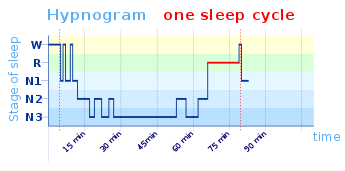
\includegraphics[width=1\textwidth]{sleep cycle.png}}
\caption{Sample hypnogram showing one sleep cycle (the first of the night) from NREM through REM \cite{WikiSleepCycle}.}
\label{fig:A3.1}
\end{figure}
\section{The Role of Sleep in Health and Disease}\label{sec:2.2}
Sleep plays a pivotal role in overall health and well-being, impacting a wide array of physiological and psychological processes. Disruptions in normal sleep patterns are associated with various health conditions.\newline
\textbf{Physical Health Implications:}

\begin{enumerate}
    \item \textbf{Cardiovascular Health:} Poor sleep quality and sleep disorders like sleep apnea are linked to an increased risk of cardiovascular diseases.Disturbances in sleep can lead to hypertension, arrhythmias, and even heart failure.\cite{Somers2008}
    \item \textbf{Metabolic Function:} Sleep deprivation can adversely affect glucose metabolism and appetite regulation, increasing the risk of obesity and type 2 diabetes.
\end{enumerate}
\textbf{Mental Health Correlations:}
\begin{enumerate}
    \item \textbf{Cognitive Functioning:} Sleep is essential for cognitive processes including learning, memory, and problem-solving.Impaired sleep can lead to deficits in these areas, impacting daily functioning and quality of life

    \item \textbf{Psychiatric Disorders:} There is a strong correlation between sleep disturbances and psychiatric conditions such as depression and anxiety.Disrupted sleep can exacerbate these conditions, creating a vicious cycle of mental health deterioration and sleep problems.

\end{enumerate}
The physiological and neurological underpinnings of sleep stages, and their role in health and disease, underscore the importance of sleep in human life. As this section of the dissertation elucidates, understanding these mechanisms is not just academically fascinating but also crucial in addressing the myriad of health issues associated with sleep disturbances.

\section{Polysomnography (PSG): An In-Depth Look}\label{2.3}
Polysomnography (PSG) is a multifaceted diagnostic tool used in sleep medicine to evaluate sleep disorders. This test records several physiological parameters during sleep, each providing crucial insights into the various aspects of sleep architecture and quality. The following is a detailed examination of each component involved in a PSG.
\subsection{Components}\label{2.3.1}
\begin{enumerate}
    \item \textbf{Electroencephalogram (EEG):} \newline
    \textbf{Function:}The primary function of EEG in PSG is to monitor and record the electrical activity of the brain. This is crucial for identifying and differentiating between the various stages of sleep (N1, N2, N3, and REM).\newline
    \textbf{Implementation:}Electrodes are strategically placed on the scalp in accordance with the 10-20 system, a standardized method for electrode placement in EEG recordings.
    \textbf{Data Interpretation:}The EEG traces display different brain wave patterns characteristic of each sleep stage. For example, theta waves for light sleep (N1), sleep spindles and K-complexes during N2, and delta waves for deep sleep (N3).
\begin{figure}[htb]
\centerline{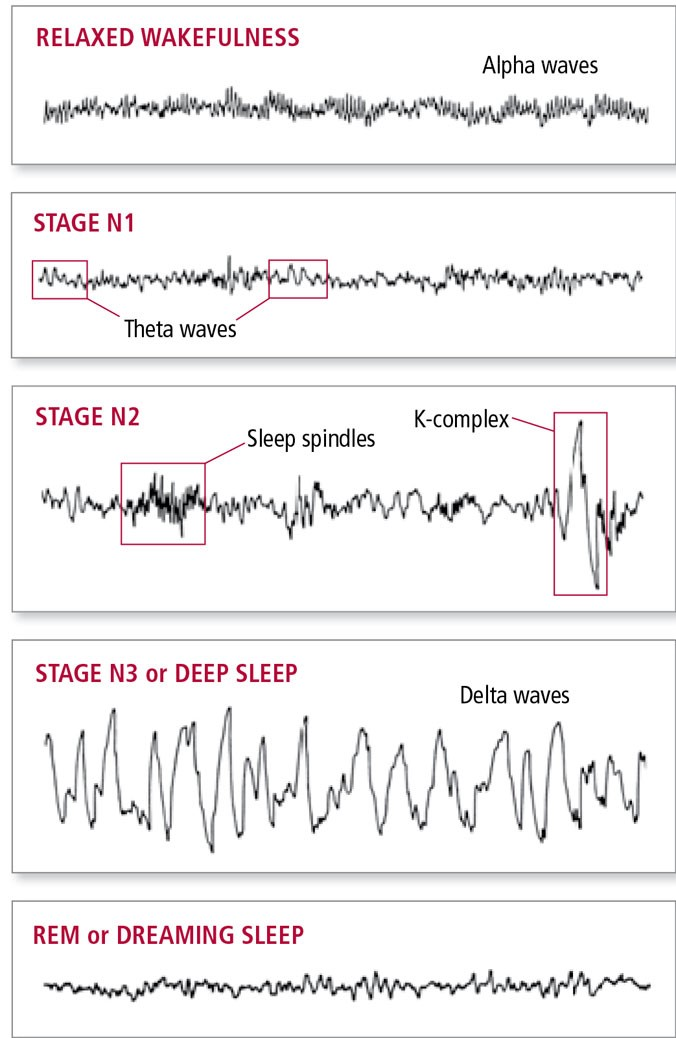
\includegraphics[height=12cm,width=15cm]{eeg.jpg}}
\caption{EEG brain wave patterns during sleep \cite{HelpGuideSleepStages}.}
\label{fig:A3.2}
\end{figure}
\item \textbf{ Electrooculogram (EOG):} \newline
\textbf{Function:} EOG records eye movements, which are particularly important for identifying REM sleep where rapid eye movements are a defining feature.
\newline \textbf{Implementation:}Electrodes are placed near the eyes, typically above and below one eye or at the outer corners of both eyes.
\newline \textbf{Data Interpretation:}The recording captures the movements of the eyes, distinguishing between the slow, rolling eye movements of Non-REM sleep and the rapid, jerky movements of REM sleep.\newline
 \begin{figure}[htb]
\centerline{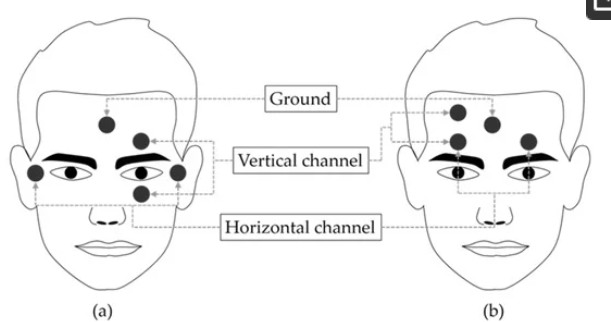
\includegraphics{eog.png}}
\caption{. Electrode placement for (a) conventional EOG and (b) proposed forehead EOG.\cite{Heo2017}.}
\label{fig:A3.3}
\end{figure}
\item \textbf{Electromyogram (EMG):}\newline
\textbf{Function:} EMG in PSG is used to measure muscle activity, which helps in detecting the reduced muscle tone during REM sleep (REM atonia) and muscle relaxation in other sleep stages.\newline
\textbf{Implementation:}Electrodes are placed on the chin to measure submental muscle tone and, in some cases, on the limbs to monitor limb movements.\newline
\textbf{Data Interpretation:} The EMG trace varies from high muscle tone during wakefulness to reduced tone in Non-REM sleep and almost complete atonia in REM sleep, except for twitches.\newline
\begin{figure}[htb]
\centerline{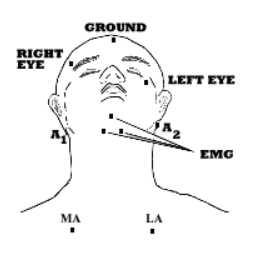
\includegraphics{emg.png}}
\caption{EMG electrode positions. \cite{CSMAClinicEMG}.}
\label{fig:A3.4}
\end{figure}

\item \textbf{ Respiratory Monitoring:}\newline
\textbf{Function:} This aspect of PSG assesses breathing patterns, effort, and airflow, crucial for diagnosing sleep-related breathing disorders.\newline
\textbf{Implementation:}Electrodes are placed on the chin to measure submental muscle tone and, in some cases, on the limbs to monitor limb movements.\newline
\begin{enumerate}
\item \textbf{Effort:}Respiratory effort is measured using belts placed around the chest and abdomen.\newline
    \begin{figure}[htb]
    \centerline{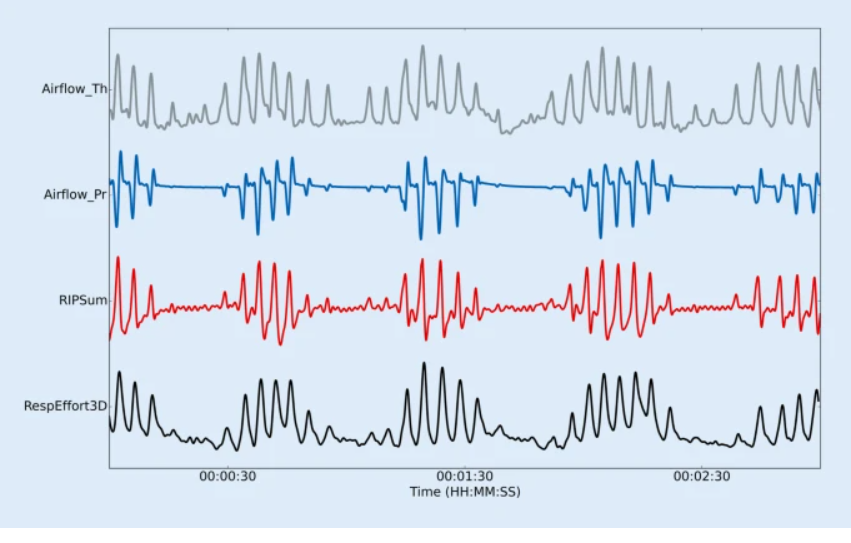
\includegraphics[height=6cm,width=15cm]{ef.png}}
    \caption{Measurement of respiratory effort in sleep by 3D camera and respiratory inductance plethysmography. \cite{eff}.}
    \label{fig:A3.4}
    \end{figure}

\item \textbf{Airflow:}Airflow is typically measured using thermistors or nasal pressure transducers placed at the nose and/or mouth.\newline

    
\item \textbf{Oxygen Saturation:}Pulse oximetry is used to monitor blood oxygen levels.

    
\end{enumerate}
\textbf{Data Interpretation:} The EMG trace varies from high muscle tone during wakefulness to reduced tone in Non-REM sleep and almost complete atonia in REM sleep, except for twitches.

\item \textbf{ Cardiac Monitoring:} \newline
\textbf{Function:} Cardiac monitoring, typically through an electrocardiogram (ECG), is included to observe heart rate and rhythm during sleep.
\newline \textbf{Implementation:}ECG electrodes are placed on the chest to record the electrical activity of the heart.
\newline \textbf{Data Interpretation:}This data can reveal any sleep-related cardiac irregularities, such as arrhythmias, which may be related to sleep apnea or other sleep disorders.\newline
 \begin{figure}[htb]
\centerline{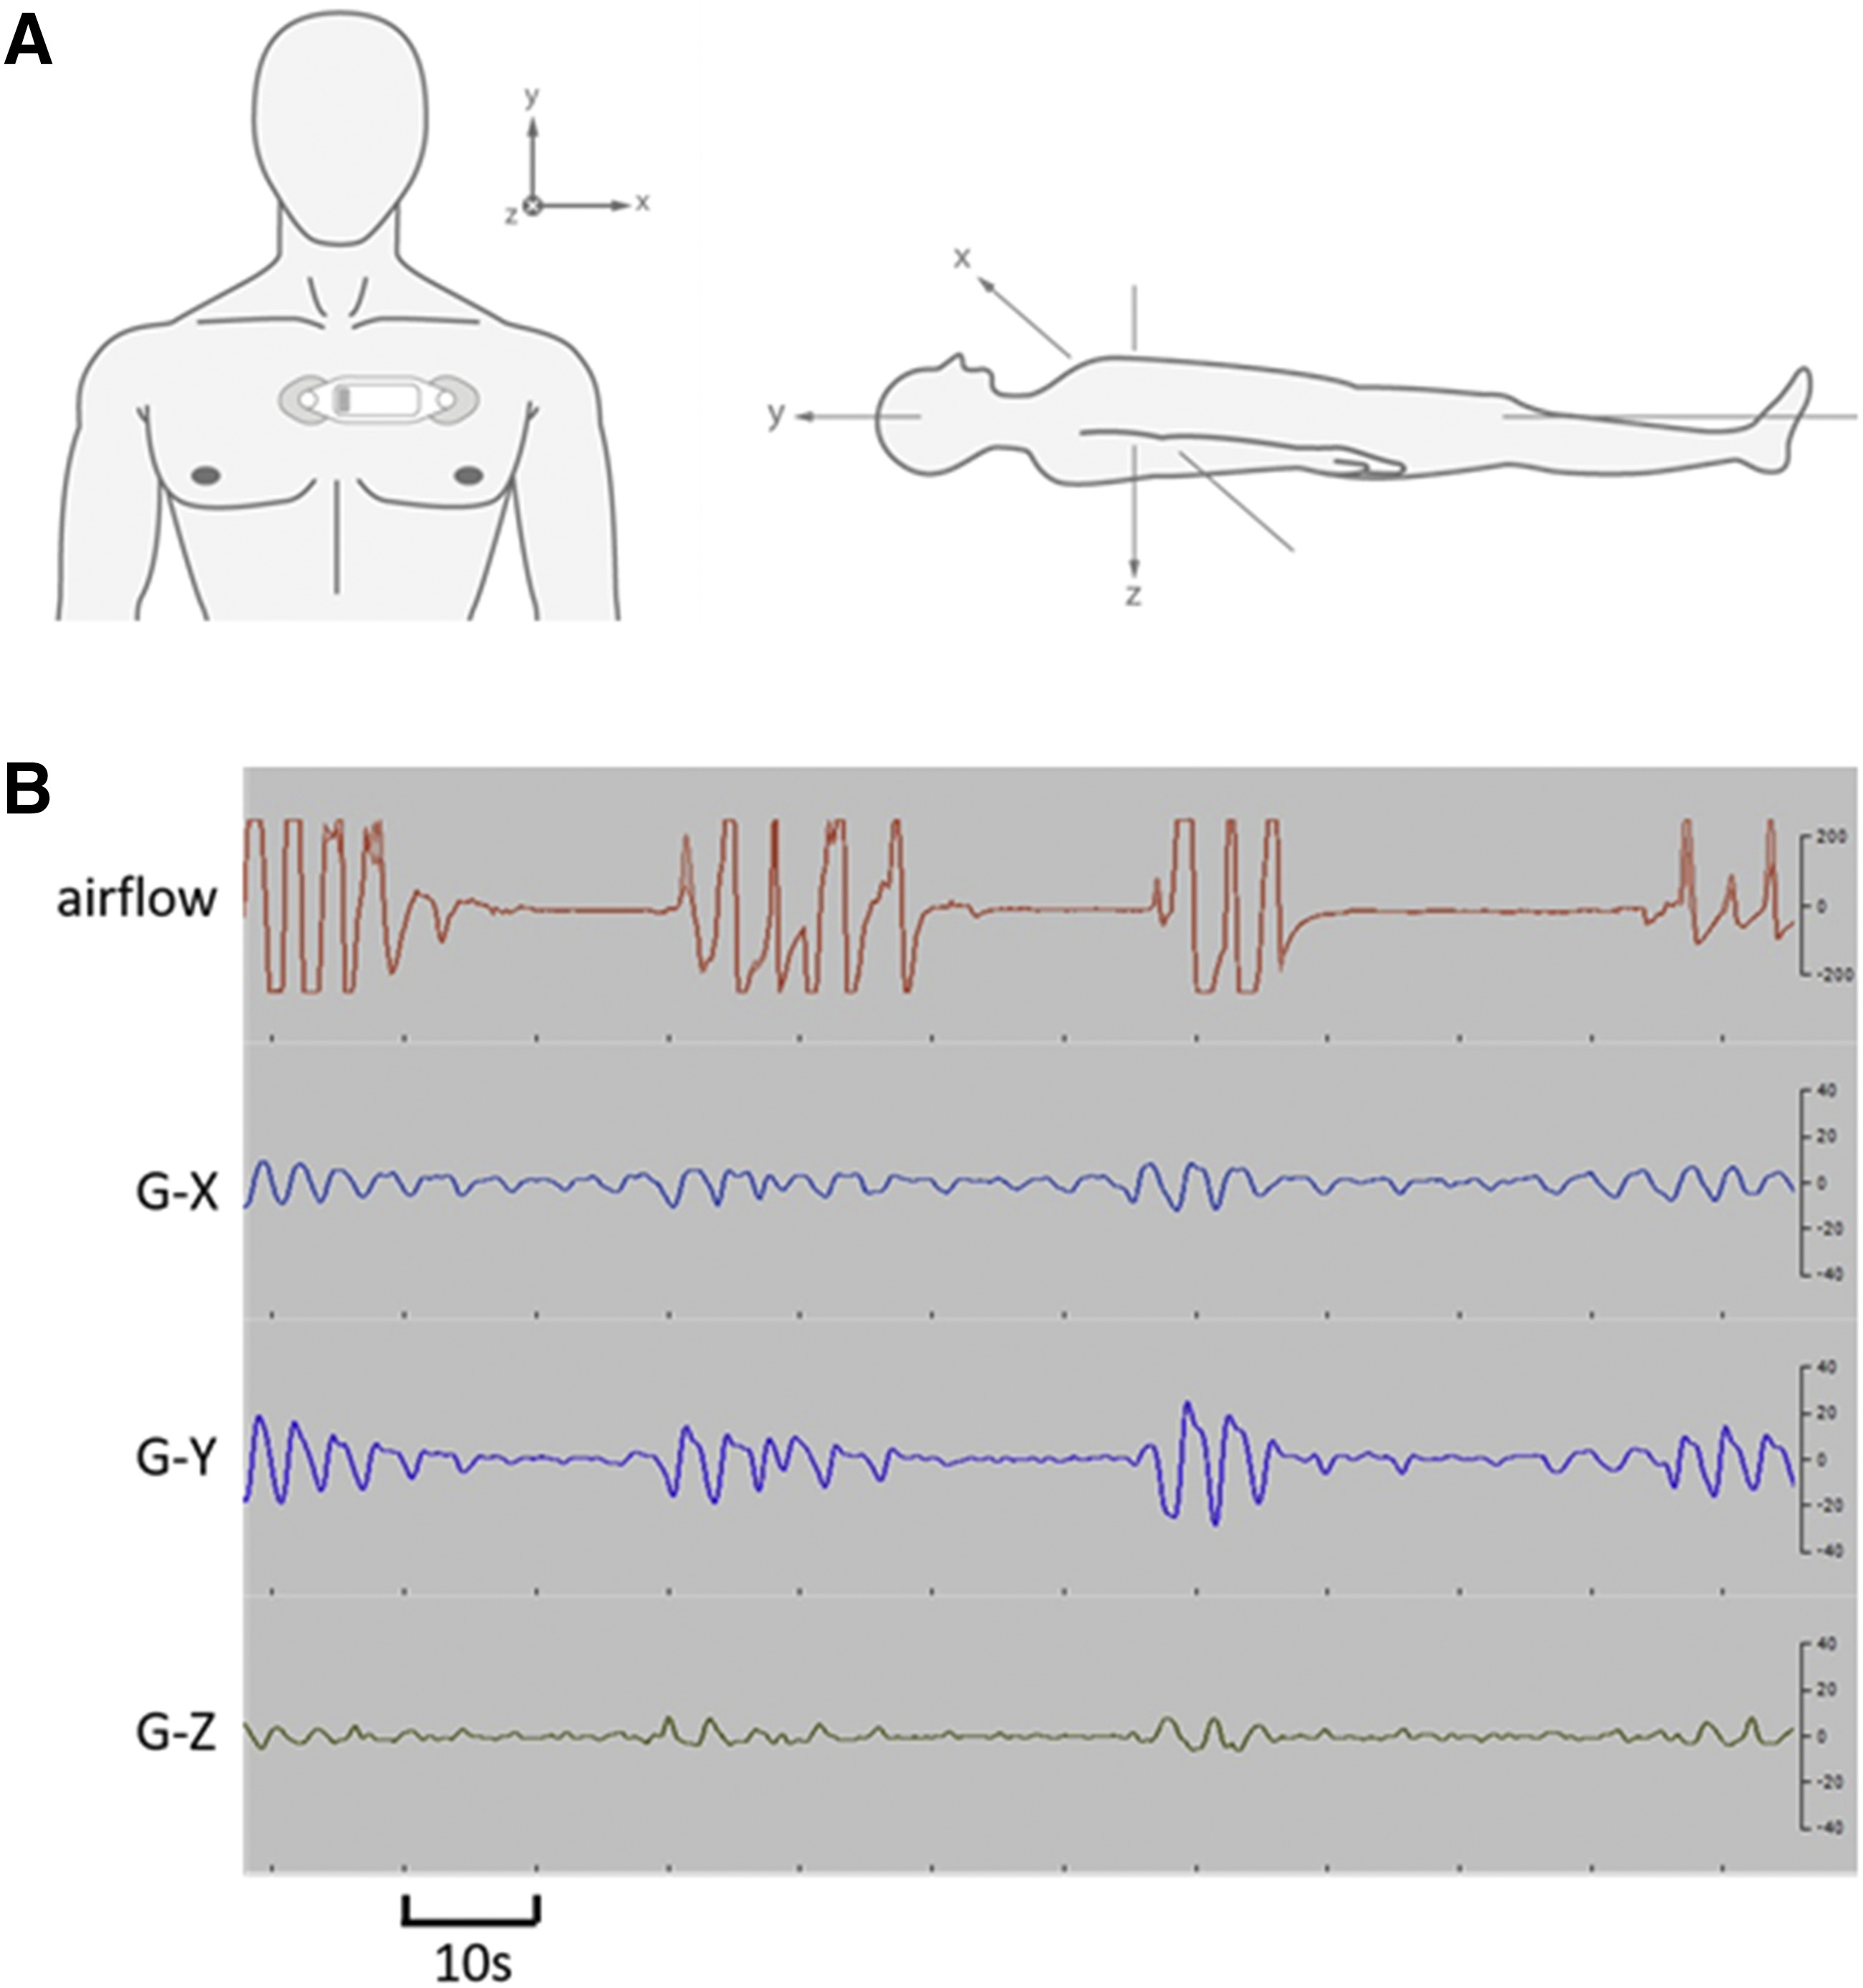
\includegraphics[height=6cm,width=15cm]{ecg.jpg}}
\caption{chest wall motion during respiratory cycles and sleep apnea events.\cite{Hsu2020}.}
\label{fig:A3.3}
\end{figure}



\end{enumerate}
The comprehensive nature of PSG, with its various components, offers a detailed view of the physiological processes occurring during sleep. This detailed recording and analysis make PSG an invaluable tool in diagnosing a wide range of sleep disorders, providing essential information for targeted treatments and interventions. As technology advances, we can anticipate more sophisticated and patient-friendly enhancements to this crucial diagnostic method.

\subsection{Procedure and Setting}\label{2.3.2}
PSG is typically conducted in a sleep laboratory, where a patient is monitored overnight. The environment is designed to be comfortable and conducive to sleep. Prior to sleep, a technician attaches the various sensors to the patient's body. The process is non-invasive, although it can be unfamiliar and slightly uncomfortable for some patients.

\subsection{Data Analysis and Interpretation:}\label{2.3.3}
The data collected during a PSG test is extensive and requires expert interpretation. Sleep specialists analyze the various waveforms and physiological signals to identify sleep stages, diagnose sleep disorders, and assess the overall quality of sleep. This analysis is pivotal in formulating a treatment plan for sleep-related conditions.
\subsection{Limitations of PSG:}\label{2.3.4}
While polysomnography (PSG) is considered the gold standard for diagnosing sleep disorders, it is not without its limitations. Understanding these limitations is crucial for researchers and clinicians in sleep medicine to interpret PSG results accurately and explore potential alternative methods.
\begin{enumerate}
    \item  \textbf{Environmental and One-Night Snapshot Limitations:} PSG typically requires an overnight stay in a sleep laboratory. This unfamiliar environment can affect the patient's normal sleep patterns, a phenomenon known as the 'first-night effect'. H W Agnew  found significant differences in sleep patterns between the first and subsequent nights in a sleep lab, indicating that the first night may not be representative of a person's typical sleep.\cite{Agnew1966}
    PSG usually provides data from only one night. Yet, sleep patterns can vary significantly from night to night. This variability can lead to misdiagnosis or an incomplete understanding of the patient's sleep disorder.

    \item \textbf{Cost and Accessibility Issues:}: The cost of a PSG test can be prohibitive for many patients.The expenses associated with the specialized equipment and staff required for PSG make it a costly diagnostic tool.
    Limited availability of sleep laboratories and trained personnel can make it difficult for patients to access PSG services.

    \item  \textbf{Invasiveness and Comfort Concerns:}: The array of electrodes and sensors used in PSG can cause physical discomfort, potentially affecting sleep quality.The invasive nature of the test can lead to anxiety or distress, further impacting sleep
\end{enumerate}
Despite its limitations, PSG remains a cornerstone in the field of sleep medicine, providing invaluable insights into sleep disorders and physiology. Its comprehensive nature allows for a detailed understanding of sleep patterns, essential for accurate diagnosis and effective treatment of sleep-related conditions. As technology evolves, there may be advancements in PSG techniques, making it more accessible and less intrusive for patients.

\section{Literature Review:}\label{sec:2.4}
In this literature review, we embark on an analytical journey through the complex domain of sleep science, with a specific focus on the delineation of sleep phases-REM and non-REM, and the emerging application of machine learning in this intricate field. The phenomenon of sleep, a fundamental yet multifaceted physiological process, has consistently piqued scientific curiosity and investigation. It offers profound insights into the intricate mechanisms of the human body and its integral relationship with overall health and mental well-being.
The early 20th century marked the advent of sleep research, gradually unraveling the layers of this enigmatic state and uncovering its pivotal role in various physiological functions. The identification of distinct sleep phases, each serving specific physiological purposes, has been a cornerstone in sleep research. Non-REM sleep, encompassing lighter stages (N1 and N2) as well as deep slow-wave sleep (N3), is intricately linked with processes such as tissue repair, memory consolidation, and hormonal regulation. Conversely, REM sleep, known for its distinct brain activity patterns and dream occurrences, is essential for cognitive processing and emotional balance. This review aims to dissect the evolution of our understanding of these phases, synthesizing a diverse array of research that underscores their physiological significance.
Central to the discourse of sleep science is the challenge of accurately and effectively monitoring sleep patterns. The field, traditionally reliant on polysomnography (PSG), a method both comprehensive and resource-intensive, faces challenges related to accessibility, cost-efficiency, and the contrived nature of sleep laboratory environments. This review intends to undertake a critical analysis of PSG, evaluating its methodologies, applications, and limitations, thereby contextualizing the emergence of more sophisticated and accessible technologies.
The advent of machine learning stands as a paradigm shift in sleep research. This technology promises to overcome the constraints of traditional sleep monitoring methods, leveraging complex algorithms to analyze extensive datasets. This review will scrutinize the intersection of machine learning with sleep science, tracing its development from initial application to its present capabilities and future potential.
An integral aspect of this technological advancement is the proliferation of wearable devices. These tools, equipped with continuous, non-intrusive data collection capabilities, have revolutionized sleep monitoring. The integration of machine learning algorithms with data from these devices, offering insights into real-world sleep patterns, has significant implications for both research and clinical practices. This review will dissect how these developments synergize, transforming our approach to sleep analysis.
Through a comprehensive examination of a broad spectrum of studies, meta-analyses, and expert opinions, this review aims to critically assess methodologies, findings, and overarching conclusions within the field, while also pinpointing areas that remain underexplored. The objective extends beyond merely summarizing existing knowledge; it seeks to connect historical discoveries with contemporary innovations and prospective advancements, underlining the dynamic and evolving nature of sleep science intertwined with machine learning.
Ultimately, this literature review strives to establish a robust foundation for the research questions and hypotheses at the heart of this dissertation. It aims to position this research within the expansive continuum of scientific inquiry into sleep, highlighting its relevance and potential contributions to the field.
\subsection{"Do Not Sleep on Traditional Machine Learning: Simple and Interpretable Techniques Are Competitive to Deep Learning for Sleep Scoring"}

In the realm of sleep science, the advent of machine learning has spurred a myriad of advancements, particularly in sleep stage classification. This paper presents a compelling case for traditional machine learning techniques, emphasizing their competitiveness against deep learning models in sleep scoring. The authors delve into various machine learning algorithms, underscoring the significance of simplicity and interpretability in clinical settings. This perspective challenges the prevalent notion in sleep research that complexity equates to superiority.\cite{VanDerDonckt2021}

The study systematically compares several machine learning models, including simpler linear models and more complex non-linear ones, to deep learning approaches. It evaluates these models based on their accuracy, computational efficiency, and ease of interpretation. The findings reveal that, in many instances, simpler models provide comparable accuracy to their more complex deep-learning counterparts. This revelation is pivotal, as it suggests that simpler models could be more suitable for real-world clinical applications due to their interpretability and lower computational demands.\cite{VanDerDonckt2021}
One of the key strengths of this paper is its comprehensive analysis of the trade-offs between model complexity and performance. The authors thoroughly discuss the implications of using complex models in clinical practice, particularly the challenges in interpreting these models and the potential risks associated with misinterpretation. They advocate for a balanced approach, where the choice of model is tailored to the specific requirements of the task, taking into consideration factors such as data availability, computational resources, and the need for interpretability.\cite{VanDerDonckt2021}
The paper also explores the potential of combining traditional and advanced machine learning techniques to create hybrid models that leverage the strengths of both approaches. This innovative idea opens up new avenues for research, suggesting that the future of sleep scoring could lie in the integration of various machine learning methodologies.\cite{VanDerDonckt2021}
In conclusion, this paper makes a significant contribution to the field of sleep research by challenging existing paradigms and advocating for a more nuanced approach to the application of machine learning in sleep scoring. Its findings have far-reaching implications, potentially influencing future research directions and clinical practices in sleep medicine.\cite{VanDerDonckt2021}

\subsection{Large-Scale Automated Sleep Staging}
Haoqi Sun's study, "Large-Scale Automated Sleep Staging," represents a significant leap in the application of machine learning to sleep research, specifically addressing the challenge of automating sleep stage classification on a large scale. This paper is particularly notable for its exploration of how machine learning can be applied to vast datasets, a common scenario in contemporary sleep studies, and its implications for both clinical practice and research.\cite{Sun2017}

The core of this research lies in its innovative use of advanced machine learning algorithms capable of handling and interpreting extensive and varied sleep data. The authors employ a range of sophisticated techniques, including deep learning models, to analyze sleep stages across a substantial dataset. This approach is critical given the increasing volume of sleep data generated by both clinical studies and wearable technology.\cite{Sun2017}

A key contribution of this paper is its demonstration of the scalability and adaptability of machine learning in sleep science. The study shows that with the correct algorithmic approach, it is possible to accurately analyze large volumes of sleep data, a task that would be impractical with traditional manual methods. This scalability is crucial for translating sleep research into practical applications, such as developing more personalized and effective treatments for sleep disorders.\cite{Sun2017}

Sun's methodology includes a meticulous validation process, ensuring that the algorithms are not only effective in large-scale data analysis but also reliable and accurate. The study's findings suggest that machine learning can significantly enhance the efficiency of sleep stage classification, making it a valuable tool for both researchers and clinicians.\cite{Sun2017}

The implications of this research are far-reaching. It paves the way for more extensive and detailed sleep studies, potentially leading to better understanding and treatment of complex sleep disorders. Furthermore, the study highlights the potential of machine learning in transforming sleep medicine into a more data-driven and precise field.\cite{Sun2017}

In summary, "Large-Scale Automated Sleep Staging" by Haoqi Sun is a pioneering work that expands the horizons of sleep research and machine learning. It provides compelling evidence of the efficacy of machine learning in analyzing large-scale sleep data, marking a significant advancement in the field.\cite{Sun2017}

\subsection{SleePyCo: Automatic Sleep Scoring with Feature Pyramid and Contrastive Learning}
Seongju Lee and colleagues' paper, "SleePyCo: Automatic Sleep Scoring with Feature Pyramid and Contrastive Learning," marks a significant stride in the field of machine learning applications in sleep research. This study introduces an innovative method for automatic sleep scoring, leveraging the strengths of feature pyramid networks and contrastive learning. The novelty of this approach lies in its ability to enhance the accuracy and efficiency of sleep stage classification, a critical aspect in diagnosing and managing sleep-related disorders.\cite{SleePyCo2021}

The research revolves around the development and implementation of the SleePyCo model, a sophisticated algorithm designed to process and interpret sleep data more effectively. The use of a feature pyramid structure allows the model to capture and integrate information at various scales, an essential aspect given the complex nature of sleep data. Additionally, the incorporation of contrastive learning techniques aids in improving the model's ability to differentiate between various sleep stages, a challenging task in traditional sleep scoring methods.\cite{SleePyCo2021}

A notable strength of the SleePyCo model is its adaptability and precision. The study demonstrates that this model can effectively handle diverse datasets, making it a potentially valuable tool for large-scale sleep studies. Furthermore, the model’s design addresses some of the key limitations of previous machine learning approaches, such as the need for large amounts of labeled data and the challenge of generalizing across different patient populations.\cite{SleePyCo2021}

The findings of Lee et al. are promising, indicating that the SleePyCo model could significantly refine the process of sleep scoring. This advancement could lead to more accurate diagnoses of sleep disorders and, consequently, more effective treatment plans. Moreover, the study opens up new possibilities for further research, particularly in exploring the integration of various machine learning techniques to enhance the analysis of sleep data.\cite{SleePyCo2021}

In summary, "SleePyCo: Automatic Sleep Scoring with Feature Pyramid and Contrastive Learning" contributes an innovative methodology to the field of sleep research. The paper stands as a testament to the potential of advanced machine learning techniques in transforming the way sleep data is analyzed and interpreted.\cite{SleePyCo2021}
\subsection{XSleepNet: Multi-View Sequential Model for Automatic Sleep Staging}
Huy Phan's "XSleepNet: Multi-View Sequential Model for Automatic Sleep Staging" presents a groundbreaking approach to sleep staging, introducing a multi-view sequential model that significantly advances the application of machine learning in sleep research. This paper is particularly noteworthy for its exploration of a sequential modeling approach, addressing the dynamic and complex nature of sleep patterns.\cite{Phan2021XSleepNet}

The XSleepNet model distinguishes itself through its multi-view framework, which allows for the integration and analysis of various types of sleep-related data. This approach acknowledges the multifaceted nature of sleep and the need for a comprehensive analysis to accurately classify sleep stages. The sequential aspect of the model is designed to capture the temporal dependencies in sleep data, a critical factor often overlooked in traditional sleep staging methods.\cite{Phan2021XSleepNet}

A significant contribution of this study is its technical innovation. The XSleepNet model employs advanced machine learning techniques, including deep learning and sequence modeling, to achieve a high level of accuracy in sleep stage classification. The model’s performance is rigorously evaluated, demonstrating its superiority over existing methods in terms of both accuracy and efficiency.\cite{Phan2021XSleepNet}

The implications of Phan's research extend beyond the realm of academic study. The XSleepNet model has the potential to revolutionize clinical practice in sleep medicine, offering a more precise and efficient tool for diagnosing sleep disorders. Additionally, the model's design paves the way for future research exploring the integration of diverse data types in sleep analysis, potentially leading to more holistic and patient-centric approaches in sleep medicine.\cite{Phan2021XSleepNet}

In conclusion, "XSleepNet: Multi-View Sequential Model for Automatic Sleep Staging" by Huy Phan  is a pivotal work that significantly enhances the understanding and application of machine learning in sleep research. The study not only demonstrates the feasibility of advanced machine learning techniques in sleep staging but also sets a new benchmark for future developments in the field.\cite{Phan2021XSleepNet}
\chapter{Methodology}\label{ch:3}
In this chapter, we outline the methodology employed for the research conducted as part of this dissertation. This section is essential as it provides the framework for the study, detailing the approaches and techniques used in the application and evaluation of machine learning models for sleep stage classification. The methodology is structured to ensure replicability, accuracy, and validity of the research findings.

\section{Data-set Selected  For the Dissertation }\label{sec:3.1}

For this research, we utilized data from the 2018 PhysioNet Challenge, a publicly accessible repository that offers a rich collection of sleep-related physiological signals. This data set is instrumental in our investigation into the application of machine learning models for sleep stage classification.
PhysioNet, an online resource for complex physiological signals, has been a critical data source for numerous studies in biomedical research. The specific dataset employed in this study is from the 2018 PhysioNet/Computing in Cardiology Challenge. The challenge focused on automatic sleep stage classification, providing a comprehensive dataset suitable for this purpose.\cite{PhysioNet2018}

The dataset includes overnight polysomnography (PSG) recordings from a diverse population, encompassing various age groups and both genders. PSG recordings, considered the gold standard in sleep research, offer a multi-dimensional view of sleep by capturing a range of physiological signals. These include electroencephalogram (EEG), electrooculogram (EOG), electromyogram (EMG), and others. Each recording in the dataset is accompanied by expert-annotated sleep stage labels, following the American Academy of Sleep Medicine (AASM) guidelines.\cite{PhysioNet2018}

\begin{table}[ht]
\centering
\caption{Dataset Composition}
\label{tab:dataset-composition}
\begin{tabular}{|l|p{10cm}|}
\hline
\textbf{Component} & \textbf{Description} \\ \hline
EEG Recordings & Multiple channels of EEG data capturing brainwave activity throughout the sleep period. \\ \hline
EOG Recordings & Recordings of eye movements, essential for identifying the REM stage of sleep. \\ \hline
EMG Recordings & Muscle activity data, particularly useful for detecting the reduced muscle tone during REM sleep. \\ \hline
Sleep Stage Labels & Expert-annotated labels for each 30-second epoch of the recordings, based on AASM standards. \\ \hline
Patient Demographics & Information on the age and gender of the subjects, contributing to the diversity of the dataset. \\ \hline
\end{tabular}
\end{table}


\begin{table}[ht]
\centering
\caption{Signal Characteristics in Sleep Study\cite{PhysioNet2018}}
\label{tab:signal-characteristics}
\begin{tabular}{|l|l|p{10cm}|}
\hline
\textbf{Signal Name} & \textbf{Units} & \textbf{Signal Description} \\ \hline
SaO2 & \% & Oxygen saturation \\ \hline
ABD & \textmu V & Electromyography, a measurement of abdominal movement \\ \hline
CHEST & \textmu V & Electromyography, measure of chest movement \\ \hline
Chin1\_Chin2 & \textmu V & Electromyography, a measure of chin movement \\ \hline
AIRFLOW & \textmu V & A measure of respiratory airflow \\ \hline
ECG & mV & Electrocardiogram, a measure of cardiac activity \\ \hline
E1-M2 & \textmu V & Electrooculography, a measure of left eye activity \\ \hline
O2-M1 & \textmu V & Electroencephalography, a measure of posterior activity \\ \hline
C4-M1 & \textmu V & Electroencephalography, a measure of central activity \\ \hline
C3-M2 & \textmu V & Electroencephalography, a measure of central activity \\ \hline
F3-M2 & \textmu V & Electroencephalography, a measure of frontal activity \\ \hline
F4-M1 & \textmu V & Electroencephalography, a measure of frontal activity \\ \hline
O1-M2 & \textmu V & Electroencephalography, a measure of posterior activity \\ \hline
\end{tabular}
\end{table}

The table 3.1 provided categorizes and describes the key components of the data set used from the 2018 PhysioNet Challenge for sleep stage classification. Each row of the table presents a different aspect of the data, highlighting its relevance and role in the context of sleep study. Here's an explanation of each element in the table:
\begin{enumerate}
    \item \textbf{EEG Recordings:}
These are recordings of brainwave activity captured using electroencephalography (EEG). EEG is a fundamental component of polysomnography and is critical for sleep analysis as it reveals the electrical activity of the brain during sleep.\newline
Different sleep stages are characterized by distinct brainwave patterns, which are essential for accurate sleep stage classification.\newline
\item \textbf{EOG Recordings:}These recordings capture eye movements using electrooculography (EOG). EOG is particularly important for identifying the Rapid Eye Movement (REM) stage of sleep.The presence and pattern of eye movements are key indicators of REM sleep, a stage associated with dreaming and distinctive brain activity.
\item \textbf{EMG Recordings::} Electromyogram (EMG) recordings measure muscle activity. In the context of sleep studies, EMG is used to detect muscle tone and movement.
EMG data helps in identifying sleep stages, particularly REM sleep, where muscle tone is significantly reduced (a phenomenon known as REM atonia).
\item \textbf{Sleep Stage Labels:}Each 30-second segment (epoch) of the recording is annotated with a sleep stage label by sleep experts. These labels follow the American Academy of Sleep Medicine (AASM) standards, which define different stages of sleep (N1, N2, N3, REM, and Wake). These labels serve as the ground truth for training and evaluating machine learning models in sleep stage classification.
\item \textbf{Patient Demographics:}This includes basic demographic information about the subjects, such as age and gender.Demographic diversity in the dataset helps ensure that the developed models are applicable and accurate across different age groups and genders, enhancing the generalizability of the research findings.


\end{enumerate}
\section{Feature Extraction}
In this dissertation, a detailed and meticulous approach to feature extraction from polysomnography (PSG) data is employed, which is pivotal for the effective application of machine learning models in sleep stage classification. The process involves several steps, each carefully executed to ensure the highest data integrity and relevance for subsequent analysis.\newline
The process begins with the loading of PSG data, which is achieved through the load data function in the script. This function efficiently handles .mat files, extracting the necessary signals from selected channels. Given the complexity of sleep data, which encompasses various physiological signals like EEG, EOG, and EMG, careful attention is paid to maintaining the integrity of the data during this stage. The signals are then transposed to align with the format required for feature extraction.\newline
Following this, the import labels function is employed to associate each 30-second epoch of the PSG data with expert-annotated sleep stage labels. This step is crucial as it lays the groundwork for a supervised learning approach, where these labels serve as the target outcomes for the machine learning models.

Given the susceptibility of PSG signals to noise and artifacts, the design filters function is utilized to create specific filters for different types of signals. This step is crucial to enhance the signal quality and ensure the reliability of the features extracted.

Subsequently, the filter signals function applies these filters to the respective signals. This function also normalizes the data, standardizing the mean and variance. This normalization is critical as it mitigates the impact of signal variability between different recordings, ensuring a level playing field for model training and evaluation.
The feature extraction phase is bifurcated into two primary components: statistical feature extraction (extract stat features) and spectral feature extraction (extract spec features).
\begin{enumerate}
    \item \textbf{Statistical Features}: This segment of the process focuses on extracting statistical parameters such as interquartile range, skewness, kurtosis, and standard deviation from the windowed signals. These features provide a quantitative overview of the distribution and variability of the physiological signals, aspects that are informative of different sleep stages.
    \item \textbf{Spectral Features:} The spectral feature extraction is particularly intricate, involving Welch's method to compute power spectral density across various frequency bands. These bands (delta, theta, alpha, sigma, beta) are pivotal in sleep science as they correspond to different sleep stages. An innovative element in this phase is the detection of sleep spindles using a continuous wavelet transform approach, which adds a layer of sophistication to the feature set.
\end{enumerate}
Once the features are extracted, they are compiled into a comprehensive dataset. A pandas DataFrame is created for each participant, which includes all the extracted features along with the corresponding sleep stage labels. This dataset forms the foundation upon which machine learning models are trained and validated.

The final step involves exporting this compiled dataset as a CSV file. This file represents the culmination of the preprocessing and feature extraction phases and serves as the input for the machine learning algorithms that follow.
The methodology adopted for feature extraction in this study is both rigorous and thorough, ensuring that the PSG data is transformed into a feature-rich format conducive to machine learning analysis. The combination of statistical and spectral features provides a multifaceted view of the sleep data, capturing various physiological dynamics that are essential for accurate sleep stage classification. This comprehensive approach to feature extraction is expected to enhance the predictive performance of the machine learning models, thereby contributing significantly to the field of sleep research.

\section{Feature Reduction Using PCA}
In addition to feature extraction, this research incorporates Principal Component Analysis (PCA) for feature reduction, specifically targeting both time-domain and frequency-domain features extracted from the polysomnography (PSG) data. 
\subsection{PCA Time Domain}
\subsubsection{Preparation and Memory Mapping}
\textbf{Memory Mapping:} Given the large size of the dataset, a memory-mapped file approach is used for efficient data handling. This method enables the processing of large arrays that do not fit entirely into memory, reducing memory consumption and enhancing computational efficiency.
\textbf{Initial Setup: }The script sets up critical parameters, including window size, sampling frequency, and channels to process. It also defines a small value, epsilon, used to check the standard deviation of the channels to ensure signal quality.
\subsubsection{Data Reshaping and Normalization}
\textbf{Reshaping and Normalization Functions:} The script includes functions to reshape data for individual channels and normalize it. Reshaping involves segmenting the continuous signal data into 30-second windows, aligning with standard sleep stage classification practices. Normalization adjusts the data to a common scale without distorting differences in the ranges of values.
\subsubsection{Batch Processing for PCA}
\textbf{Batch Processing:} To manage the large volume of data, the script processes the data in batches. This approach allows for handling substantial datasets by dividing them into smaller, more manageable segments.
\textbf{PCA on Each Batch:} Principal Component Analysis is performed on each batch of data. The PCA model is configured to reduce the feature set to a specified number of principal components, capturing the most significant variance in the data while reducing dimensionality.
\subsubsection{Aggregation and Averaging of PCA Coefficients}
\textbf{Aggregating PCA Coefficients}: After processing each batch, the PCA coefficients (principal components) are aggregated. These coefficients represent the transformed feature space where the dimensions are the principal components that best explain the variance in the data.
\textbf{Averaging Across Batches:} The PCA coefficients from all batches are averaged to obtain a generalized set of components. This step ensures that the feature reduction is representative of the entire dataset and not biased towards any specific batch.
\subsubsection{Output and Storage}
\textbf{DataFrame Creation:} The averaged PCA coefficients are stored in a pandas DataFrame for easy access and manipulation. Each column in the DataFrame corresponds to a channel in the PSG data, now represented in the reduced feature space.
\textbf{Exporting PCA Coefficients:} The final step involves exporting the averaged PCA coefficients to a CSV file. This file contains the reduced feature set that will be used for training and validating the machine learning models.
\newline \newline
The inclusion of PCA in the methodology serves a dual purpose. Firstly, it significantly reduces the dimensionality of the feature space, making the machine learning models more computationally efficient. Secondly, by focusing on the principal components, the models are likely to capture the most relevant aspects of the data, potentially enhancing their predictive accuracy. This approach is particularly advantageous in the context of sleep stage classification, where the high dimensionality of raw PSG data can pose challenges in model training and performance.
\subsection{PCA Frequency Domain}
The methodology for frequency-domain feature reduction in this research involves a sophisticated process of Principal Component Analysis (PCA) applied to the frequency-domain features extracted from polysomnography (PSG) data.
\subsubsection{Preparation and Memory Mapping}
\textbf{Memory Mapping:} To efficiently manage the large volume of PSG data, a memory-mapped file system is utilized. This allows for handling data that surpasses the available memory, ensuring efficient data processing and access.

\textbf{Setting Parameters:} The script sets essential parameters such as window size, sampling frequency, and the selected channels for analysis. An epsilon value is defined to check the standard deviation of the signals, ensuring the quality and reliability of the data.

\subsubsection{Data Reshaping and Normalization for Frequency Analysis}
Reshaping for Frequency Analysis: The script includes a function reshape onesubj freq to reshape and prepare data specifically for frequency-domain analysis. This involves segmenting the continuous signals into 30-second epochs and performing Welch's power spectral density estimation.

\textbf{Normalization}: Each frequency-domain feature is normalized to ensure consistency across the dataset. This normalization involves applying a logarithmic transformation to the power spectral density estimates, followed by scaling and centering.

\subsubsection{Batch Processing and PCA}
\textbf{Processing PSG Data:} The script iteratively processes PSG data from each subject, handling cases where signal quality is compromised (indicated by a standard deviation below the epsilon threshold).

\textbf{PCA Application:} Principal Component Analysis is then performed on the collected frequency-domain data. The PCA model reduces the number of features to a specified number, focusing on retaining the most significant components that capture the core variance in the data.

\subsubsection{Output and Storage}
\textbf{Storing PCA Scores and Coefficients:} The PCA scores (transformed data) and the PCA coefficients (principal components) are stored in pandas DataFrames. The scores represent the data in the reduced feature space, while the coefficients provide insight into the feature contribution to each principal component.

\textbf{Exporting Results}: The final PCA scores and coefficients are exported as CSV files for further analysis. This step ensures that the reduced feature set is readily available for machine learning model training and validation.
\newline\newline
The inclusion of PCA in the frequency-domain feature analysis offers several advantages. Firstly, it significantly condenses the feature space, making it more manageable and computationally efficient for machine learning algorithms. Secondly, by concentrating on principal components, the models can focus on the most informative aspects of the frequency-domain data, potentially improving their predictive accuracy. This approach is especially beneficial in sleep stage classification, where the frequency characteristics of physiological signals play a crucial role. Through this methodology, the research aims to capture the essence of the frequency-domain features while reducing complexity and enhancing model performance.
\section{Machine Learning}
In this dissertation, we employ a suite of advanced machine learning algorithms to classify sleep stages based on the features extracted from polysomnography data. The chosen algorithms include XGBoost, Logistic Regression, CatBoost, and Random Forest. Each of these algorithms is well-regarded in the machine learning community for its performance in various classification tasks. The following sections provide an overview and rationale for selecting each of these algorithms.
\subsection{XGBoost (eXtreme Gradient Boosting)}
XGBoost stands out as a highly efficient and scalable implementation of gradient boosting. It has gained popularity due to its performance in numerous machine learning competitions and applications. XGBoost is known for its speed and performance, particularly in handling large and complex datasets, which makes it well-suited for sleep stage classification where the datasets are often substantial and multidimensional.\cite{Chen2016}.

One of the key features of XGBoost is its ability to handle sparse data and its robustness to overfitting, partly due to the regularization components in its objective function. It also offers flexibility in defining custom optimization objectives and evaluation criteria, making it adaptable to various data characteristics and research requirements. The algorithm's effectiveness in capturing complex patterns in data makes it a strong candidate for analyzing the intricate relationships in sleep data \cite{Chen2016}.
\subsection{Logistic Regression}
Logistic Regression, despite its simplicity compared to more complex models, remains a staple in statistical modeling and machine learning. It's particularly valued for its interpretability and efficiency, especially in binary classification tasks. In the context of sleep stage classification, Logistic Regression serves as a benchmark to assess the performance of more complex algorithms.\cite{Hosmer2013}

The algorithm models the probability of a binary outcome based on a linear combination of the input features. Its simplicity allows for a clear understanding of the influence of each feature on the predicted outcome, an aspect crucial for clinical interpretability in sleep research.\cite{Hosmer2013}

\subsection{CatBoost}
CatBoost is a relatively recent addition to the ensemble of tree-based machine learning algorithms. It has been designed to provide high performance with categorical data, although it performs equally well with numerical data. One of the key strengths of CatBoost is its robust handling of categorical features, automatically determining useful representations for them, which can be particularly beneficial in sleep data that often comprises both categorical and continuous variables.\cite{Prokhorenkova2018}

CatBoost's algorithmic advancements reduce overfitting and improve generalization, making it a valuable tool in our sleep stage classification task. Its efficient implementation and support for GPU acceleration also make it suitable for handling large datasets typically associated with sleep studies.\cite{Prokhorenkova2018}

\subsection{Random Forest}
Random Forest is an ensemble learning method known for its high accuracy, robustness, and ease of use. It operates by constructing a multitude of decision trees during training and outputting the class that is the mode of the classes of the individual trees. Random Forest can handle a large number of input variables without variable deletion, which is essential for our research given the multidimensional nature of PSG data.\cite{Breiman2001}

A significant advantage of Random Forest in sleep stage classification is its ability to reduce overfitting while maintaining the accuracy of large datasets. It also offers insights into the importance of different features for classification, aiding in understanding the underlying patterns in sleep data.\cite{Breiman2001}

\newline\newline
The selection of these diverse machine learning algorithms aims to provide a comprehensive analysis of the extracted features from PSG data. By comparing the performance of these different models, we can identify the most effective approach for classifying sleep stages, considering both accuracy and interpretability, which are critical in clinical applications.

\section{Model Training and Validation Pipeline}
This section of the dissertation elaborates on the methodical approach adopted for the training and validation of various machine learning algorithms, including XGBoost, Logistic Regression, CatBoost, and Random Forest, in the context of sleep stage classification. This pipeline is meticulously designed to ensure a robust assessment of each model's performance, accounting for the nuances and complexities inherent in sleep data.
\subsection{Overview of the Pipeline}
The pipeline is built on a foundation of rigorous data preparation, cross-validation, and performance evaluation. Its flexibility allows for the interchangeable use of different machine learning algorithms while maintaining a consistent framework for training and assessment.
\subsubsection{Data Preparation and Sampling}
\textbf{Participant Selection:} The dataset encompasses a diverse range of participants. For each iteration of model training and validation, a random sample of participant IDs is selected. This randomization is crucial to prevent model bias and ensure the generalizability of the findings.

\textbf{Data Segregation:} The complete dataset is divided into subsets based on the chosen participant IDs, creating a focused dataset for each iteration. This step is vital in maintaining data integrity and avoiding information leakage between the training and testing phases.

\subsubsection{Train-Test Split and Preprocessing}
\textbf{Splitting Strategy:} A 70-30 train-test split is employed, wherein 70\% of the data is used for training the model, and the remaining 30\% is reserved for testing. This ratio is chosen to provide a substantial training dataset while ensuring enough data is available for an accurate assessment of model performance.

\textbf{Data Preprocessing:} The features (X) and labels (y) are extracted from the dataset. The features undergo a preprocessing step where missing values are handled (filled with zeros), and label values are adjusted appropriately. This preprocessing is crucial for model compatibility and to ensure accurate predictions.

\textbf{Feature Scaling:} The features are scaled using the StandardScaler, normalizing them to have a mean of zero and a standard deviation of one. Scaling is critical, particularly in datasets with features of varying magnitudes, to prevent any single feature from dominating the learning process.

\subsubsection{Cross-Validation and Model Training}
\textbf{KFold Cross-Validation:} To validate the model's effectiveness and its generalizability, a KFold cross-validation with 5 splits is implemented. This approach ensures that each subset of the data is used both for training and testing, thereby providing a comprehensive evaluation of the model's performance.
\textbf{Iterative Model Training:} In each fold, the model is trained on the scaled training data. The use of multiple machine learning algorithms within the same pipeline underscores the versatility of the approach. Each algorithm, with its unique strengths and characteristics, is evaluated under the same rigorous conditions.

\subsubsection{Performance Metrics}
\textbf{Accuracy:} The accuracy metric assesses the overall correctness of the model predictions. It is a fundamental metric but is complemented by more nuanced metrics to provide a fuller picture of model performance.

\textbf{F1-Score: }The F1-Score is particularly useful in imbalanced datasets. It combines precision and recall into a single metric, balancing the trade-off between false positives and false negatives.

\textbf{Recall and Precision:} These metrics provide insights into the model's ability to correctly classify positive cases (recall) and the proportion of true positive predictions (precision). They are critical in medical applications like sleep stage classification, where missing or incorrectly labeling a stage can have significant implications.
\subsubsection{Aggregation and Analysis of Results}
\textbf{Mean Metric Calculation:} Post each cross-validation fold, the mean of each performance metric is calculated. This mean provides a consolidated view of the model's performance in that particular fold.

\textbf{Overall Performance Assessment:} The pipeline is repeated for multiple iterations, with each iteration involving a different set of randomly selected participants. The aggregation of results across these iterations offers a robust estimate of the model's performance, mitigating the impact of any anomalies or biases present in a single iteration.

\textbf{Comparative Analysis:} The final step involves a comparative analysis of the performance metrics across different machine learning models. This comparison is instrumental in identifying the most effective model for sleep stage classification, taking into account factors like accuracy, reliability, and computational efficiency.
\newline\newline
This comprehensive training and validation pipeline serves as the backbone of the research methodology. Its systematic approach, encompassing data preparation, model training, cross-validation, and performance evaluation, ensures that the findings are reliable and replicable. The pipeline's adaptability to various machine learning algorithms makes it a valuable framework, not only for this research but also as a reference for future studies in sleep stage classification and related areas.
\section{Results}
In this section of my dissertation, I present a detailed analysis of the performance of four machine learning models - XGBoost, CatBoost, SVM, and Logistic Regression - in the context of sleep stage classification. The evaluation is conducted under two distinct experimental conditions: one with a 4-channel feature extraction followed by PCA, and the other utilizing a more extensive 13-channel feature extraction without PCA. The results of these experiments provide crucial insights into the efficacy of these algorithms in handling complex sleep data.
\begin{table}[ht]
\centering
\caption{Model Performance Scores(4 Channels Feature  Extraction + PCA)}
\label{tab:model-performance}
\begin{tabular}{|l|c|}
\hline
\textbf{Model} & \textbf{Accuracy (\%)} \\ \hline
XGBoost & 80.19 \\ \hline
CatBoost & 80.66 \\ \hline
SVM & 80.04 \\ \hline
Logistic Regression & 74.30 \\ \hline
\end{tabular}
\end{table}
\begin{table}[ht]
\centering
\caption{Model Performance Scores(13 Channels Feature  Extraction)}
\label{tab:performance-metrics}
\begin{tabular}{|l|c|c|c|c|}
\hline
\textbf{Model} & \textbf{Accuracy\%} & \textbf{F1-Score} & \textbf{Recall} & \textbf{Precision} \\ \hline
XGBoost & 81.66 & 0.8195 & 0.7951 & 0.8568 \\ \hline
CatBoost &80.59 & 0.8027 & 0.7776 & 0.8413 \\ \hline
SVM & 81.66 & 0.8195 & 0.7951 & 0.8568 \\ \hline
Logistic Regression & 49.26 & 0.3164 & 0.3104 & 0.4659 \\ \hline
\end{tabular}
\end{table}
\section{Experiment 1: 4 Channels Feature Extraction + PCA (Table 3.3)}
\subsection{Model Performance:}

\textbf{XGBoost:} Exhibited an accuracy of 80.19\%. This high accuracy reflects XGBoost's robustness in handling dimensionally reduced data and its efficiency in managing the nuances of sleep stages.\newline
\textbf{CatBoost:} Surpassed XGBoost slightly with an accuracy of 80.66\%. This marginally higher accuracy could be attributed to CatBoost’s handling of categorical features, which might be playing a significant role even in this reduced feature set.\newline
\textbf{SVM:} Showed a competitive accuracy of 80.04\%. SVM's performance is particularly noteworthy, given its relative simplicity compared to the ensemble methods. This suggests its capability in capturing essential patterns in the sleep data even after dimensionality reduction.\newline
\textbf{Logistic Regression:} Lagged behind with an accuracy of 74.30\%. This lower performance could be due to Logistic Regression’s linear nature, which might struggle with the complexity embedded in the sleep data, even in its dimensionally reduced form.

\subsection{Analysis:}

The results from this experiment highlight the strengths of ensemble methods in sleep stage classification, especially in scenarios where feature dimensionality is reduced. The slight edge of CatBoost over XGBoost could be indicative of its specialized handling of the dataset's inherent characteristics. SVM's comparable performance suggests its potential as a simpler yet effective alternative. Logistic Regression’s lower accuracy points to its limitations in dealing with reduced feature sets in complex classification tasks like sleep stage classification.

\section{Experiment 2: 13 Channels Feature Extraction (Table 3.4)}
\subsection{Model Performance:} 

\textbf{XGBoost and SVM:} Both models achieved an accuracy of 81.66\%, with an F1-Score of 81.95\%, Recall of 79.51\%, and Precision of 85.68\%. These results are indicative of their effectiveness in handling multi-dimensional data, capturing intricate patterns in the more extensive feature set derived from the 13-channel data.\newline
\textbf{CatBoost:} Showed a balanced performance with an accuracy of 80.59\%, F1-Score of 80.27\%, Recall of 77.76\%, and Precision of 84.13\%. CatBoost’s performance, while slightly lower than XGBoost and SVM, demonstrates its competency in managing complex data structures.\newline
\textbf{Logistic Regression:} Significantly underperformed with an accuracy of 49.26\%, F1-Score of 31.64\%, Recall of 31.04\%, and Precision of 46.59\%. This substantial drop in performance across all metrics suggests that Logistic Regression is less suited for high-dimensional data, likely due to its inability to model complex, non-linear relationships inherent in such data.

\subsection{Analysis:}

The results from the 13-channel feature extraction experiment underscore the capability of ensemble methods and SVM in handling high-dimensional data, evident from their high scores across all metrics. The consistency of XGBoost and SVM in both accuracy and other metrics indicates their robustness and reliability. CatBoost’s balanced performance across metrics makes it a viable option, particularly in scenarios where trade-offs between different metrics are considered. The stark underperformance of Logistic Regression highlights its limitations in contexts involving complex, multi-dimensional data.

\section{Comparative Analysis}
Comparing the results from both experiments, it is evident that the ensemble methods and SVM consistently outperform Logistic Regression, irrespective of the feature extraction method employed. The use of PCA in the 4-channel data did not significantly alter the relative performance of the models compared to the 13-channel data. This suggests that the additional channels in the 13-channel setup provide valuable information that is not fully captured in the reduced feature set post-PCA.


\chapter{Conclusions}\label{ch:concl}
This dissertation has provided an in-depth exploration of the application of various machine learning models in the classification of sleep stages. Through a methodical approach to data preparation, feature extraction, model training, and validation, the research has sought to determine the most effective techniques for interpreting the complex data derived from polysomnography.

The experimental results indicate that ensemble methods, such as XGBoost and CatBoost, as well as SVM, are particularly effective in sleep stage classification. These models demonstrate robustness and high accuracy in both the reduced feature set post-PCA and the more comprehensive multi-channel feature extraction. Logistic Regression, while offering benefits in terms of simplicity and interpretability, shows limitations in handling the complexity and high dimensionality inherent in sleep data.

One of the key findings of this research is the importance of feature selection and extraction in sleep stage classification. The comparison between the 4-channel reduced feature set and the 13-channel comprehensive feature extraction illustrates that while PCA is effective in reducing dimensionality and noise, the additional information captured in multi-channel data can be crucial for accurate classification.

The research also highlights the critical role of proper data preprocessing and cross-validation in developing reliable and generalizable machine learning models. By employing a systematic approach to data scaling, splitting, and model evaluation, the study ensures the robustness of its findings.

This dissertation contributes to the broader understanding of how machine learning can be applied in the field of biomedical signal processing, particularly in sleep medicine. The insights gained from this study could have significant implications for clinical practices, potentially leading to more accurate and efficient methods for diagnosing sleep disorders.

Moreover, the methodologies and findings of this research provide a foundation for future studies in this area. Future research could explore the integration of additional physiological signals, the application of newer or more complex machine learning models, and the development of real-time sleep stage classification systems.

In conclusion, this research underscores the potential of machine learning in enhancing our understanding of sleep patterns and disorders. The findings of this study contribute valuable knowledge to the field and pave the way for further innovations in sleep stage classification using machine learning techniques.









\begin{thebibliography}{999}

%%% Bibliography items should be below this here %%%

\bibitem{Berry2012}
R.B. Berry, R. Budhiraja, D.J. Gottlieb, et al.
\newblock Rules for scoring respiratory events in sleep: update of the 2007 AASM Manual for the Scoring of Sleep and Associated Events. Deliberations of the Sleep Apnea Definitions Task Force of the American Academy of Sleep Medicine.
\newblock {\em J Clin Sleep Med}, 8(5):597--619, 2012.
\newblock Published 2012 Oct 15. doi:10.5664/jcsm.2172


\bibitem{Steriade2006}
M.~Steriade.
\newblock Grouping of brain rhythms in corticothalamic systems.
\newblock {\em Neuroscience}, 137(4):1087--1106, 2006.
\newblock doi:10.1016/j.neuroscience.2005.10.029

\bibitem{VanCauter2000}
E.~Van Cauter, R.~Leproult, and L.~Plat.
\newblock Age-related changes in slow wave sleep and REM sleep and relationship with growth hormone and cortisol levels in healthy men.
\newblock {\em JAMA}, 284(7):861--868, 2000.
\newblock doi:10.1001/jama.284.7.861

\bibitem{Aserinsky1953}
E.~Aserinsky and N.~Kleitman.
\newblock Regularly occurring periods of eye motility, and concomitant phenomena, during sleep.
\newblock {\em Science}, 118(3062):273--274, 1953.
\newblock doi:10.1126/science.118.3062.273

\bibitem{Hobson2000}
J.A. Hobson, E.F. Pace-Schott, and R. Stickgold.
\newblock Dreaming and the brain: toward a cognitive neuroscience of conscious states. [published correction appears in Behav Brain Sci 2001 Jun;24(3):575].
\newblock {\em Behav Brain Sci}, 23(6):793--1121, 2000.
\newblock doi:10.1017/s0140525x00003976

\bibitem{Siegel2005}
J.M. Siegel.
\newblock Clues to the functions of mammalian sleep.
\newblock {\em Nature}, 437(7063):1264--1271, 2005.
\newblock doi:10.1038/nature04285


\bibitem{Somers2008}
V.K. Somers, D.P. White, R. Amin, et al.
\newblock Sleep apnea and cardiovascular disease: an American Heart Association/american College Of Cardiology Foundation Scientific Statement from the American Heart Association Council for High Blood Pressure Research Professional Education Committee, Council on Clinical Cardiology, Stroke Council, and Council On Cardiovascular Nursing. In collaboration with the National Heart, Lung, and Blood Institute National Center on Sleep Disorders Research (National Institutes of Health). [published correction appears in Circulation. 2009 Mar 31;119(12):e380].
\newblock {\em Circulation}, 118(10):1080--1111, 2008.
\newblock doi:10.1161/CIRCULATIONAHA.107.189375
\bibitem{Sun2017}
Haoqi Sun, Jian Jia, Balaji Goparaju, Guang-Bin Huang, Olga Sourina, Matt Travis Bianchi, M Brandon Westover.
\newblock Large-Scale Automated Sleep Staging.
\newblock Affiliations: Energy Research Institute @ NTU, Interdisciplinary Graduate School, Nanyang Technological University, Singapore; Fraunhofer IDM @ NTU, Nanyang Technological University, Singapore; School of Mathematics, Northwest University, Xi'an, Shaanxi, China; Massachusetts General Hospital, Neurology Department, Boston, MA; School of Electrical and Electronic Engineering, Nanyang Technological University, Singapore.
\newblock {\em Sleep}, 2017.
\newblock DOI: \url{10.1093/sleep/zsx139}
\newblock PMID: 29029305
\newblock PMCID: PMC6251659
\bibitem{Phan2021XSleepNet}
Huy Phan, Oliver Y. Chén, Minh C. Tran, Philipp Koch, Alfred Mertins, and Maarten De Vos.
\newblock XSleepNet: Multi-View Sequential Model for Automatic Sleep Staging.
\bibitem{WikiSleepCycle}
Wikipedia contributors. 
\newblock ``Sleep cycle.''
\newblock \textit{Wikipedia, The Free Encyclopedia}, 
\newblock Wikipedia, The Free Encyclopedia, 25 Nov. 2023.
\newblock Web. 1 December 2023.
\newblock URL: \url{https://en.wikipedia.org/wiki/Sleep_cycle}

\bibitem{HelpGuideSleepStages}
HelpGuide.org.
\newblock ``Stages of Sleep: REM Sleep, Deep Sleep, and Circadian Rhythm.''
\newblock \textit{HelpGuide}, in collaboration with Harvard Health,
\newblock Web. 1 December 2023..
\newblock URL: \url{https://www.helpguide.org/harvard/biology-of-sleep-circadian-rhythms-sleep-stages.htm}

\bibitem{Heo2017}
J. Heo, H. Yoon, and K.S. Park.
\newblock A Novel Wearable Forehead EOG Measurement System for Human Computer Interfaces.
\newblock {\em Sensors (Basel, Switzerland)}, 17(7):1485, 2017.
\newblock \url{https://doi.org/10.3390/s17071485}

\bibitem{CSMAClinicEMG}
CSMA Clinic.
\newblock EMG electrode position.
\newblock \textit{Comprehensive Sleep Medicine Associates}, 
\newblock Web. [Access date].
\newblock URL: \url{https://csma.clinic/HTML/EMG.htm}


\bibitem{eff}
Carmina Coronel.
\newblock Measurement of respiratory effort in sleep by 3D camera and respiratory inductance plethysmography.
\newblock {\em Sensors (Basel, Switzerland)}, 17(7):1485, 2017.
\newblock \url{https://doi.org/10.3390/s17071485}

\bibitem{Entropy2021}
Riccardo Pernice,Tatjana Loncar-Turukalo,Gorana Mijatović
.
\newblock Assessment of Cardiorespiratory Interactions during Apneic Events in Sleep via Fuzzy Kernel Measures of Information Dynamics.
\newblock {\em Entropy}, 23(6):698, May 2021.
\newblock DOI: \url{10.3390/e23060698}
\newblock License: CC BY 4.0

\bibitem{Hsu2020}
Ying-Shuo Hsu, Tien-Yu Chen, Dean Wu, Chia-Mo Lin, Jer-Nan Juang, Wen-Te Liu, et al.
\newblock Screening of obstructive sleep apnea in patients who snore using a patch-type device with electrocardiogram and 3-axis accelerometer.
\newblock {\em J Clin Sleep Med}, 2020.
\newblock DOI: \url{10.5664/jcsm.8462}
\newblock PMID: 32267228

\bibitem{Agnew1966}
H.W. Agnew Jr, W.B. Webb, and R.L. Williams.
\newblock The first night effect: an EEG study of sleep.
\newblock {\em Psychophysiology}, 2(3):263--266, 1966.
\newblock DOI: \url{10.1111/j.1469-8986.1966.tb02650.x}

\bibitem{VanDerDonckt2021}
J. Van Der Donckt, J. Van Der Donckt, E. Deprost, N. Vandenbussche, M. Rademaker, G. Vandewiele, S. Van Hoecke.
\newblock Do Not Sleep on Linear Models: Simple and Interpretable Techniques Outperform Deep Learning for Sleep Scoring.
\newblock URL: \url{https://ar5iv.org/abs/2207.07753}

\bibitem{SleePyCo2021}
Seongju Lee, Yeonguk Yu, Seunghyeok Back, Hogeon Seo, and Kyoobin Lee.
\newblock SleePyCo: Automatic Sleep Scoring with Feature Pyramid and Contrastive Learning.

\bibitem{Chen2016}
T. Chen and C. Guestrin.
\newblock XGBoost: A scalable tree boosting system.
\newblock In \textit{Proceedings of the 22nd ACM SIGKDD International Conference on Knowledge Discovery and Data Mining}, 2016.
\bibitem{PhysioNet2018}
PhysioNet.
\newblock PhysioNet/CinC Challenge 2018: Training/Test Sets.
\newblock Retrieved [Access Date], from \url{https://archive.physionet.org/pn3/challenge/2018/}
\bibitem{Hosmer2013}
D.W. Hosmer Jr, S. Lemeshow, and R.X. Sturdivant.
\newblock \textit{Applied Logistic Regression}.
\newblock John Wiley \& Sons, 2013.

\bibitem{Prokhorenkova2018}
L. Prokhorenkova, G. Gusev, A. Vorobev, A.V. Dorogush, and A. Gulin.
\newblock CatBoost: unbiased boosting with categorical features.
\newblock In \textit{Advances in Neural Information Processing Systems}, 2018.


\bibitem{Breiman2001}
L. Breiman.
\newblock Random forests.
\newblock \textit{Machine Learning}, 45(1):5--32, 2001.


\end{thebibliography}





\end{document}

